\documentclass[10pt,letterpaper]{article}
\usepackage[margin=0.72in]{geometry}
\usepackage[T1]{fontenc}
\usepackage{lmodern,microtype,booktabs,graphicx,amsmath,xcolor,hyperref}
\hypersetup{colorlinks=true,urlcolor=blue,linkcolor=blue,pdftitle={Check forecast publication deadlines before scoring scheduling errors},pdfauthor={James N. Jean IV}}
\setlength{\parindent}{0pt}
\setlength{\parskip}{6pt}
\renewcommand{\arraystretch}{1.18}
\pagestyle{plain}
\newcommand{\AheadMae}{857.6}
\newcommand{\AheadRmse}{1028.4}
\newcommand{\AheadMse}{1057583.7}
\newcommand{\AheadBias}{320.0}
\newcommand{\AheadWape}{1.6}
\newcommand{\AheadUnder}{1494.8}
\newcommand{\NoonMae}{619.3}
\newcommand{\NoonRmse}{821.8}
\newcommand{\NoonMse}{675401.2}
\newcommand{\NoonBias}{126.8}
\newcommand{\NoonWape}{1.2}
\newcommand{\NoonUnder}{1329.3}
\newcommand{\EndMae}{338.0}
\newcommand{\EndRmse}{443.6}
\newcommand{\EndMse}{196821.8}
\newcommand{\EndBias}{156.2}
\newcommand{\EndWape}{0.6}
\newcommand{\EndUnder}{1323.4}
\newcommand{\FirstAhead}{591.3}
\newcommand{\FirstNoon}{668.6}
\newcommand{\FirstForecast}{60082.7}
\newcommand{\FirstActual}{58287.8}
\newcommand{\FirstError}{1794.9}
\newcommand{\SecondForecast}{62009.4}
\newcommand{\SecondActual}{60005.8}
\newcommand{\SecondError}{2003.6}
\newcommand{\ThirdForecast}{60442.6}
\newcommand{\ThirdActual}{61064.3}
\newcommand{\ThirdError}{-621.7}
\newcommand{\FourthForecast}{62604.6}
\newcommand{\FourthActual}{63406.9}
\newcommand{\FourthError}{-802.3}
\newcommand{\FifthForecast}{60878.1}
\newcommand{\FifthActual}{59702.8}
\newcommand{\FifthError}{1175.3}
\newcommand{\NorthAhead}{7.6}
\newcommand{\NativeChecks}{101139}
\newcommand{\NativeRows}{2242}
\newcommand{\ProjectedRows}{4320}
\newcommand{\NumericChecks}{48524}
\newcommand{\Comparisons}{3240}
\newcommand{\PeakRows}{135}
\newcommand{\FigureChecks}{597}
\begin{document}
{\Large\bfseries Check the forecast deadline before scoring a scheduling decision\par}
{\large A five-day ERCOT archive audit and implementation exercise\par}
James N. Jean IV \hfill 30 October 2026\\
Independent reproducibility study. Not peer reviewed.

\textbf{Decision.} A team reviewing a day-ahead load decision needs the forecast file eligible at its decision deadline. A later file can make the reported error smaller while answering a different question.

\textbf{Measured finding.} Across 120 system hours on 25--29 October 2026, mean absolute error is \AheadMae{} MW at a prior-day noon cutoff, \NoonMae{} MW at same-day noon and \EndMae{} MW at the end of the operating day. Both same-day selectors miss the prior-day deadline for all 120 hours. End-of-day documents were published after 115 of those hourly intervals had ended.

\begin{center}
\begin{tabular}{lrrr}\toprule
Captured document cutoff & MAE (MW) & RMSE (MW) & WAPE (\%)\\\midrule
Prior-day noon, eligible & \AheadMae & \AheadRmse & \AheadWape\\
Same-day noon, late & \NoonMae & \NoonRmse & \NoonWape\\
End of operating day, late & \EndMae & \EndRmse & \EndWape\\\bottomrule
\end{tabular}
\end{center}
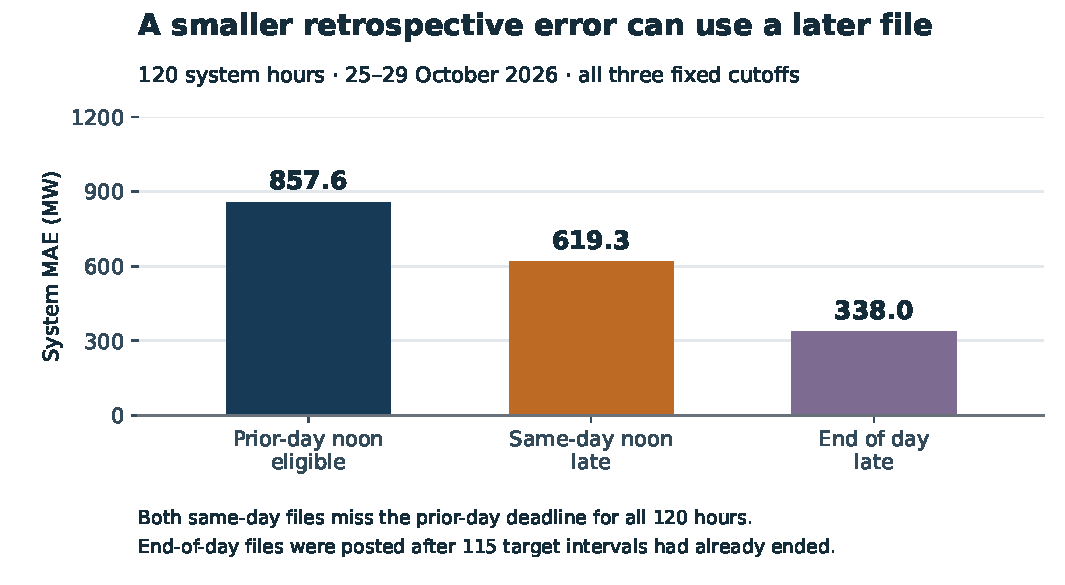
\includegraphics[width=\linewidth]{images/system_cutoffs.pdf}

\textbf{Practical action.} Retain the publication identifier and declared publication time with every forecast. Select against an explicit aware deadline; reject late, stale or tied inputs before scoring. Report all planned comparisons.

\textbf{Limits.} This is a descriptive audit of five adjacent days, not a reserve-policy improvement or seasonal forecast evaluation. Current archive metadata do not independently prove immutable original content or delivery to a historical analyst. Noon is an authored study cutoff, not a claim about ERCOT's actual scheduling deadline.
\newpage
{\Large\bfseries Bind the value to its publication record\par}

The public forecast product NP3-561-CD and actual-load product NP6-345-CD provide paired CSV/XML reports. Metadata and one non-cohort pair from each product were inspected before fixing the protocol. The forecast schema pair was published on 30 October at 19:30 Central; the actual schema pair covers 30 September. Target-day values were captured after the protocol commit.

The fixed cohort contains every hour of five operating days, eight weather zones and the independently reported system total. All cohort hours are UTC$-$05:00 with native DSTFlag=N. The implementation rejects unexpected repeated-hour flags rather than claiming general daylight-saving support. Source files also contain other dates; only the prespecified target-day cells enter this analysis.

For each day, each selector chooses the latest CSV report at or before its cutoff, requires age at most 90 minutes, and requires a unique XML pair at the same declared publication time. Actuals use the earliest available pair published the next day. They are retrospective reference labels, not proven settlement-final or revision-free measurements. Both forecast and actual retrieval times are retained separately from their publication timestamps.

The resulting 32 documents represent 16 distinct CSV/XML pairs. Their retained ZIP archives total 246224 bytes. An independent archive check passes 260 conditions. Separate parsers reconcile \NativeRows{} native CSV rows and the paired XML, source identities, SQLite as-of selectors and \ProjectedRows{} projected source rows through \NativeChecks{} finite conditions. Counts include repeated checks on related records; they are not independent statistical observations.

For forecast $f_i$, actual $a_i$ and error $e_i=f_i-a_i$:
\[
 \operatorname{MAE}=\frac{\sum |e_i|}{n},\quad
 \operatorname{MSE}=\frac{\sum e_i^2}{n},\quad
 \operatorname{RMSE}=\sqrt{\operatorname{MSE}},\quad
 \operatorname{WAPE}=\frac{\sum|e_i|}{\sum a_i}.
\]
Here all actual loads are positive. A zero denominator is unavailable in the authored fixture. Signed bias is mean forecast minus actual; maximum underprediction is $\max(0,\max_i(a_i-f_i))$. Loads and errors are MW; MSE is MW$^2$. These are load-error descriptions, not reserve requirements.

\begin{center}
\begin{tabular}{lrrr}\toprule
Cutoff & MSE (MW$^2$) & Bias (MW) & Max. under (MW)\\\midrule
Prior-day noon & \AheadMse & \AheadBias & \AheadUnder\\
Same-day noon & \NoonMse & \NoonBias & \NoonUnder\\
End of day & \EndMse & \EndBias & \EndUnder\\\bottomrule
\end{tabular}
\end{center}

Exact source sums and products use Decimal arithmetic; divisions and square roots use 60 digits. The independent checker joins source facts in SQLite, reconstructs sufficient sums as exact fractions and evaluates derived quantities at 80 digits, with absolute tolerance$10^{-45}$. The maximum observed derived difference is$3.334\times10^{-54}$ after rounding upward for display. Native quantities, sufficient sums, identities and timing flags agree exactly. No fitted model, hyperparameter search, seed, confidence interval or significance test applies.
\newpage
{\Large\bfseries Keep the unfavorable day and peak timing visible\par}

The same-day noon file has a larger system MAE on 25 October: \FirstNoon{} MW versus \FirstAhead{} MW at the eligible prior-day cutoff. A lower five-day pooled error does not describe every day. The end-of-day comparison is also ineligible for that prior-day decision, regardless of its error.

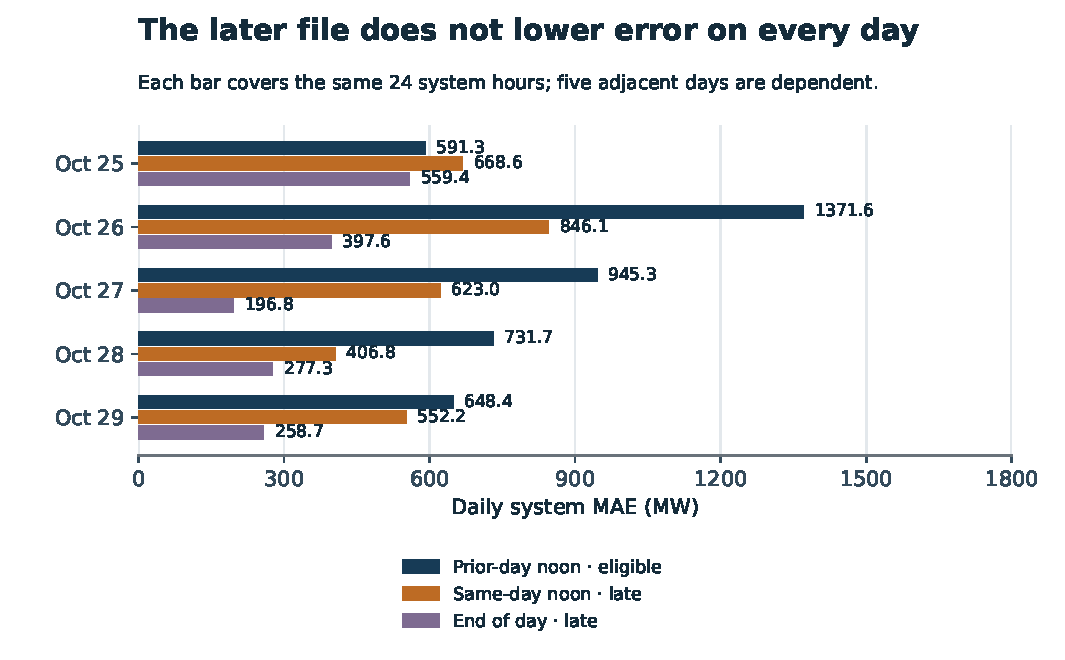
\includegraphics[width=\linewidth]{images/daily_system_errors.pdf}

The eligible prior-day forecast peak includes the actual-peak hour on three of the five days. These are five dependent descriptive cases, not an estimated reliability rate. The code retains all peak-hour ties rather than selecting an arbitrary first maximum.

\begin{center}
\begin{tabular}{lrrr}\toprule
Operating day & Forecast peak (MW) & Actual peak (MW) & Difference (MW)\\\midrule
25 October & \FirstForecast & \FirstActual & \FirstError\\
26 October & \SecondForecast & \SecondActual & \SecondError\\
27 October & \ThirdForecast & \ThirdActual & \ThirdError\\
28 October & \FourthForecast & \FourthActual & \FourthError\\
29 October & \FifthForecast & \FifthActual & \FifthError\\\bottomrule
\end{tabular}
\end{center}

The exports retain all \Comparisons{} hourly comparisons, 27 pooled metric rows, 135 daily metric rows and \PeakRows{} peak cases. No day, zone or cutoff was dropped after scores appeared. Forecast values in an after-interval file can incorporate later information or revisions; this audit does not identify their internal construction or describe them as prospective forecasts of an elapsed interval.
\newpage
{\Large\bfseries Preserve the zone-level result\par}

The published system total is a separate source series. It is not added to its zones, and the study does not assume exact equality between the reported total and the sum of rounded regional fields. North's prior-day WAPE is \NorthAhead{}\%, compared with the system's \AheadWape{}\%. Related zones share weather and system conditions; these are not nine independent replications.

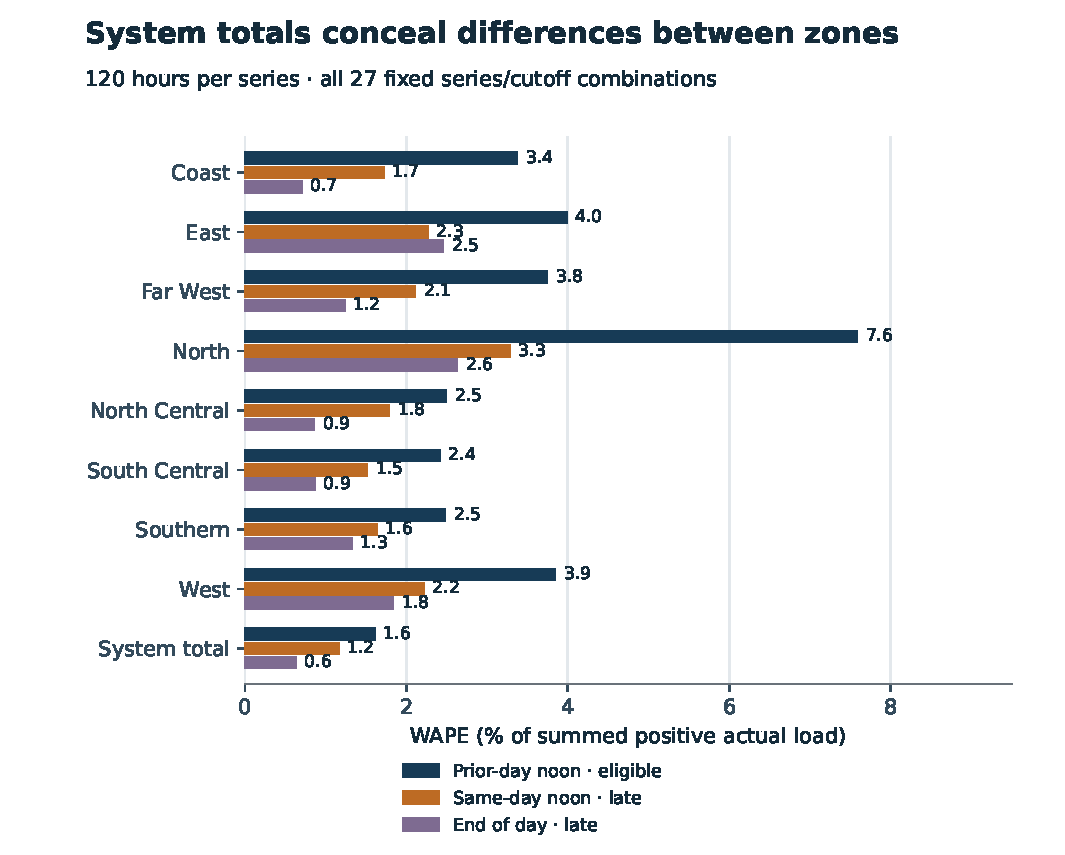
\includegraphics[width=\linewidth]{images/all_series_wape.pdf}

WAPE uses summed absolute error over summed positive actual load within each series. All 27 planned series/cutoff cases share the same 120 hours. The scale is common and begins at zero. No sampling uncertainty is encoded by the bars. Figures retain 45 bound values, 360 checked SVG coordinates, 45 numeric labels and nine asset hashes; \FigureChecks{} conditions pass. Current PNGs and the assembled manuscript were inspected separately for layout.
\newpage
{\Large\bfseries A deadline guard that can be inspected and replayed\par}

The local command below uses the captured metadata list and returns document 1290329758, published 24 October 2026 at 11:30 Central, with age 1800 seconds. A file first published after noon is never substituted when no eligible file exists.

\begin{quote}\ttfamily\small
python src/deadline.py --deadline "2026-10-24T12:00:00-05:00"
\end{quote}

Twenty-two authored fixture methods cover exact deadline equality, late-only inputs, stale and missing reports, publication ties, duplicate identities, naive timestamps, equivalent offsets, malformed numeric loads, missing/duplicate hours, unsupported DST flags, closed-form metrics and peak ties. Three saved exercise cases pass six conditions: one real archive selection, an authored late-only rejection and an authored stale-input rejection. This is finite local software evidence; no production user, deployment or operating decision was observed.

The source cohort was committed before error scoring. Fifty-three source/method dependencies were committed in a freeze before the first descriptive score command. Data were already present; this ordering does not establish analyst blindness. All planned case exports pass \NumericChecks{} independent arithmetic, lineage and timing conditions.

Two separate full-history Git clones ran the analysis replay in CPython 3.10.11 and 3.12.14. Each reproduced six result files byte for byte and left 40 public source files unchanged, with no source requests. The replay covers the saved data, native pairing, calculations, fixtures and guard. It does not reacquire private ZIP archives or establish historical delivery. The full release command also checks current figure and paper bindings.

\begin{quote}\ttfamily\small
python src/replay.py --out /external/replay-directory
\end{quote}

\textbf{What remains unestablished.} The original EIA-930/NOAA proposal for learned residual corrections, calibrated intervals, held seasons and balancing-authority transfer remains unexecuted. Five autumn days in one system cannot establish those claims. A real deployment needs monitored ingest time, immutable retained content, verified operational deadlines and sustained prospective evaluation. No reserve saving, financial benefit, causal effect, new estimator or scientific-priority claim follows.

\textbf{Sources and rights.} ERCOT, \href{https://www.ercot.com/mp/data-products/data-product-details?id=NP3-561-CD}{Seven-Day Load Forecast by Weather Zone}, \href{https://www.ercot.com/mp/data-products/data-product-details?id=NP6-345-CD}{Actual System Load by Weather Zone}, and \href{https://www.ercot.com/help/terms}{Terms of Use}, inspected 30 October 2026. Paragraph 5 permits raw public data in compilations, charts and analyses. Data and original graphics here are attributed; no ERCOT logo or endorsement is implied. Agency reports are supplied without an accuracy warranty. Only this reviewed independent study manuscript is public; separate formal-publication projects remain private.
\end{document}
